\section{Flappy Karel MDP}

There is a hot new mobile game on the market called Flappy Karel, where Karel the robot must dodge the red pillars of doom and flap its way to the green pasture. Karel needs your help in finding the best path to take in different scenarios. Below we have described Flappy World and Karel's capabilities in more detail:

\textbf{Flappy World}

\begin{itemize}
  \item Each square on the Flappy World grid represents a single state which Karel may occupy
  \item Squares shaded in red represent terminal states, taking an action from these squares will provide Karel with a reward of $r_{r}$ and end the episode
  \item Squares shaded in green represent the goal state and are also terminal, taking an action from these squares will provide Karel with a reward of $r_{g}$ and end the episode.
  \item Squares left unshaded represent non-terminal states, taking an action from these squares will provide Karel with a reward of $r_{s}$
\end{itemize}

\textbf{Karel's Movement} 

\begin{itemize}
  \item Karel can move right and up (e.g. starting from square 2 Karel can move to square 8)
  \item Karel can move right and down (e.g. starting from square 2 Karel can move to square 10)
  \item There are walls in each version of Flappy World represented by thicker edges. If a move taken by Karel runs into a wall this will result in Karel falling down one square (e.g. going in any direction from square 30 results in falling to square 31)
  \item Actions are deterministic and always succeed unless they cause Karel to run into a wall
\end{itemize}

\textbf{Assumptions (unless we have specified otherwise)}
\begin{itemize}
  \item Discount factor $\gamma = 0.9$
  \item $r_{g} = +5$
  \item $r_{r} = -5$
\end{itemize}


We will consider the following two variations of the described environment in the upcoming questions (Flappy World \ref{fig:fig1} and Flappy World \ref{fig:fig2}).  



\begin{figure}[ht]
\begin{subfigure}{.5\textwidth}
  \centering
  % include first image
  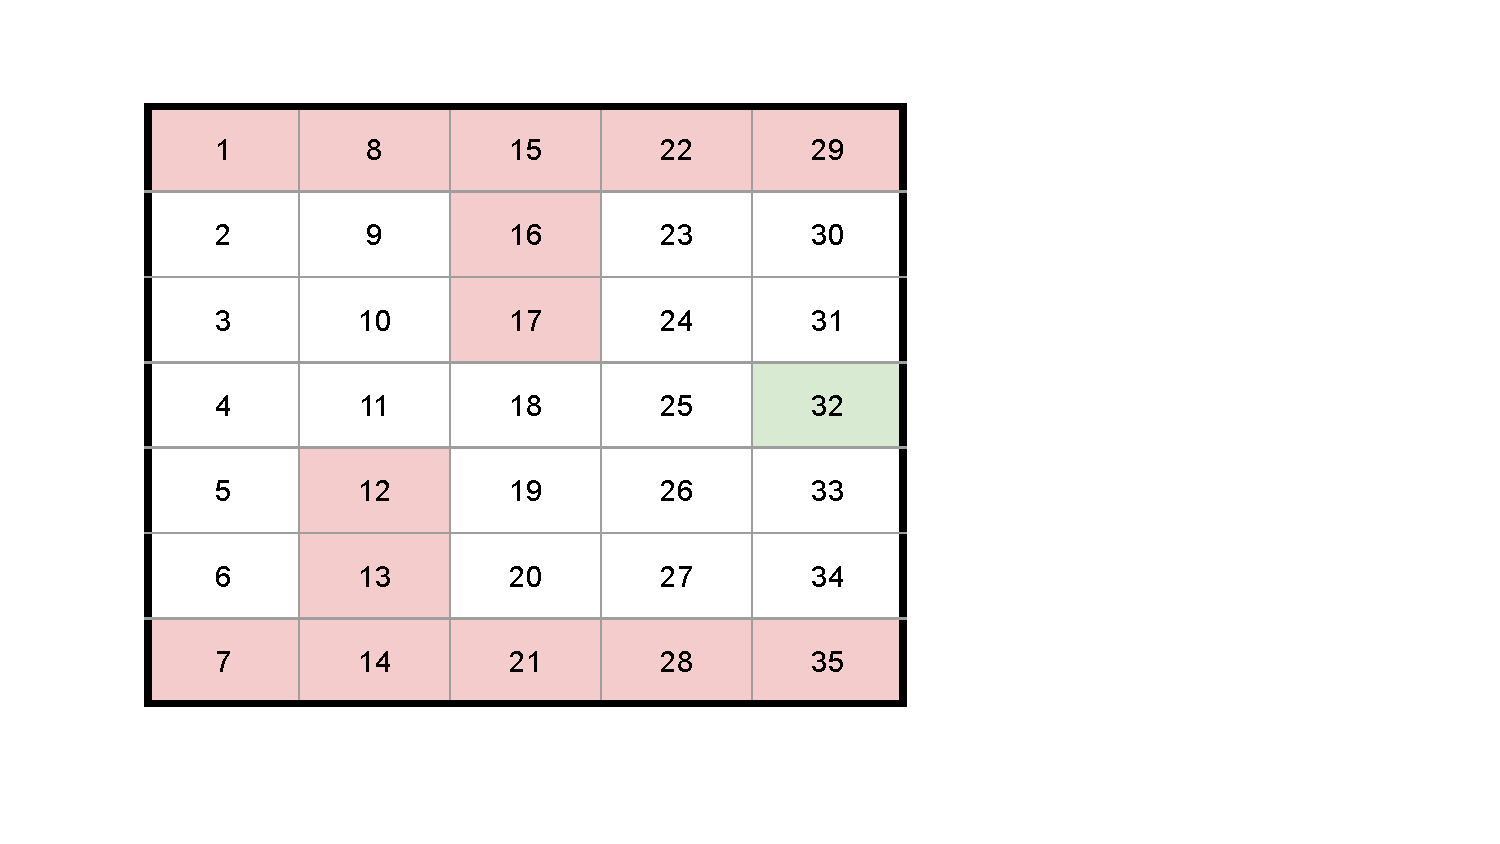
\includegraphics[width=.8\linewidth]{images/FlappyWorld1.pdf}  
  \caption{Flappy World 1}
  \label{fig:fig1.a}
\end{subfigure}
\begin{subfigure}{.5\textwidth}
  \centering
  % include second image
  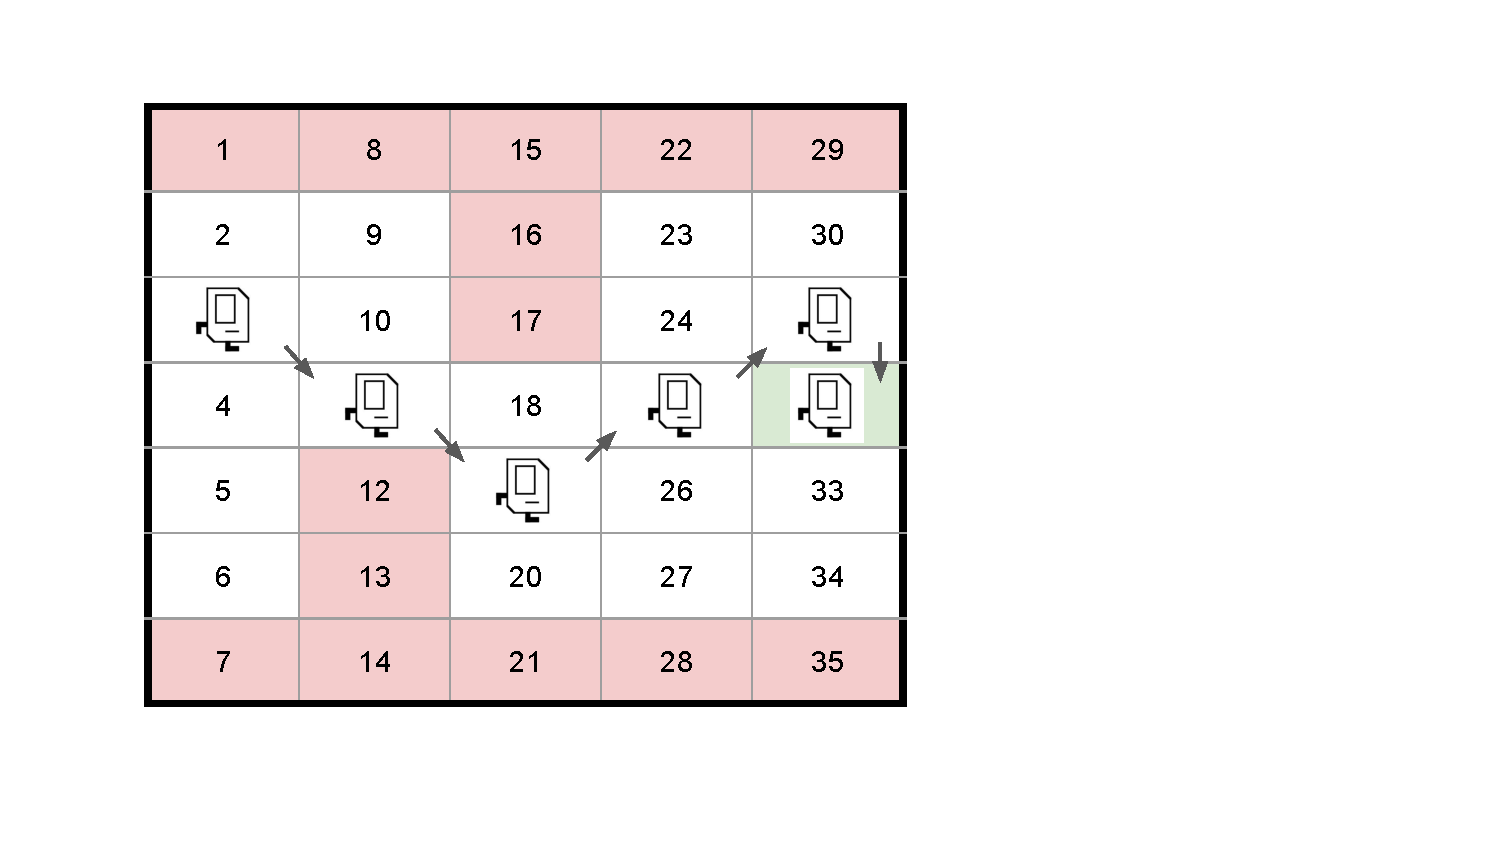
\includegraphics[width=.8\linewidth]{images/FlappyWorld1_.pdf}  
  \caption{A successful run by Karel in Flappy World 1}
  \label{fig:fig1.b}
\end{subfigure}
\caption{}
\label{fig:fig1}
\end{figure}

\clearpage 

\begin{enumerate}[(a)]

  \input{01-flappy-karel/01-fw1-optimal-policy}

  \input{01-flappy-karel/02-fw1-optimal-value-function}

  \input{01-flappy-karel/03-fw2-optimal-value-function}

  \input{01-flappy-karel/04-value-function-derivation}

  \item \points{1e}

Please refer to question 1.1 of the Gradescope online assessment ~A1 (Quiz)~.

\clearpage

\end{enumerate}